\documentclass[12pt, a4paper]{article}

%<<<===Переменные титульного листа
\newcommand{\kafedra}{ИИТ} % Кафедра X

\newcommand{\numberOfLab}{15} % Лабораторная работа №X
\newcommand{\semestr}{2} % За X семестр
\newcommand{\distiplina}{ОАиП} % По дисциплине <<X>>
\newcommand{\labTitle}{Динамические структуры: списки и деревья} % Тема: <<X>>

% Выполнил
\newcommand{\kurs}{1} % Студент X курса
\newcommand{\group}{ПО-4 (1)} % группы X
\newcommand{\labAuthor}{Галанин П. И.} % X

% Проверил
\newcommand{\teacherStatus}{ст. преподаватель} % X
\newcommand{\teacher}{Хацкевич М. В.} % X

\newcommand{\labDate}{Брест, 2020} % X
%===>>>

%<<<===
\usepackage{../../../sty/encoding} % кодировка
\usepackage{../../../sty/titlePage} % титульный лист
\usepackage{../../../sty/fields} % поля
\usepackage{../../../sty/imgs} % картинки
\usepackage{../../../sty/code} % исходный код
\usepackage{../../../sty/labData} % для лабораторной
%===>>>

\begin{document}

%<<<===Титульный лист
\maketitle
\setcounter{page}{2}
%===>>>

%<<<===Содержание
\renewcommand{\contentsname}{Содержание}
\tableofcontents
\newpage
%===>>>

%<<<===ЛР
\labheading
%===>>>

%<<<===Цель
\labgoal{Приобретение навыков работы с динамической памятью и указателями на С. Изучение принципов работы с динамическими структурами данных: списками и деревьями.}
%===>>>

%<<<===Ход Работы
\labreport
%===>>>

%<<<===Условие
\begin{center}
    Вариант 24
\end{center}
Написать программу, обеспечивающую редактирование трех списков слов: добавление, удаление, очистку, просмотр. Реализовать функцию замены всех вхождений второго списка в первый на копию третьего список, подсчитать количество замен.
%===>>>

%<<<===Исходный код
\section{Исходный код}
\subsection{main()}

Блок-схема на рисунке \ref{fig:main}.

\begin{figure}[pht]
    \center{
        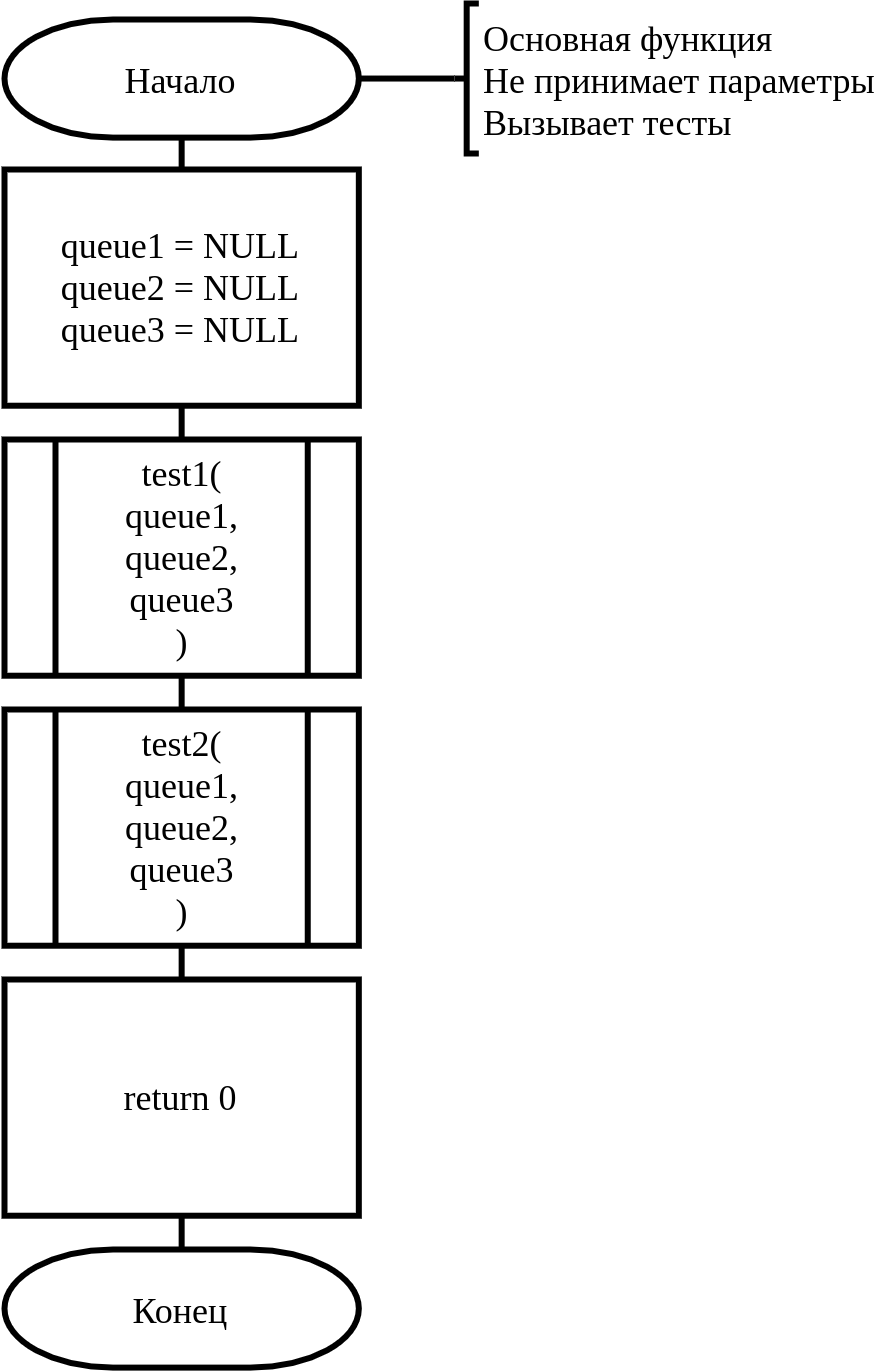
\includegraphics[]{../src/main.png}
    }
    \caption{main()}
    \label{fig:main}
\end{figure}

\lstinputlisting[
    language=C,
    name=main.c
]{../src/main.c}

\lstinputlisting[
    language=C,
    name=main.h
]{../src/main.h}

% = = = = = = = = = = =

\subsection{lab()}

%Блок-схема на рисунке \ref{fig:lab}.

%\begin{figure}[ht]
%    \center{
%        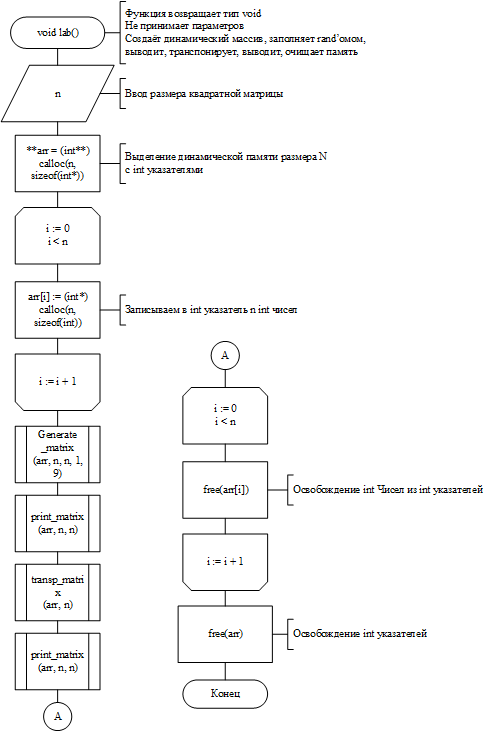
\includegraphics[]{../src/lab/lab.png}
%    }
%    \caption{lab()}
%    \label{fig:lab}
%\end{figure}

\lstinputlisting[
    language=C,
    name=lab.c
]{../src/lab/lab.c}

\lstinputlisting[
    language=C,
    name=main.h
]{../src/lab/lab.h}

% = = = = = = = = = = =

\subsection{add\_element\_to\_node()}

Блок-схема на рисунке \ref{fig:add_element_to_node}.

\begin{figure}[pht]
    \center{
        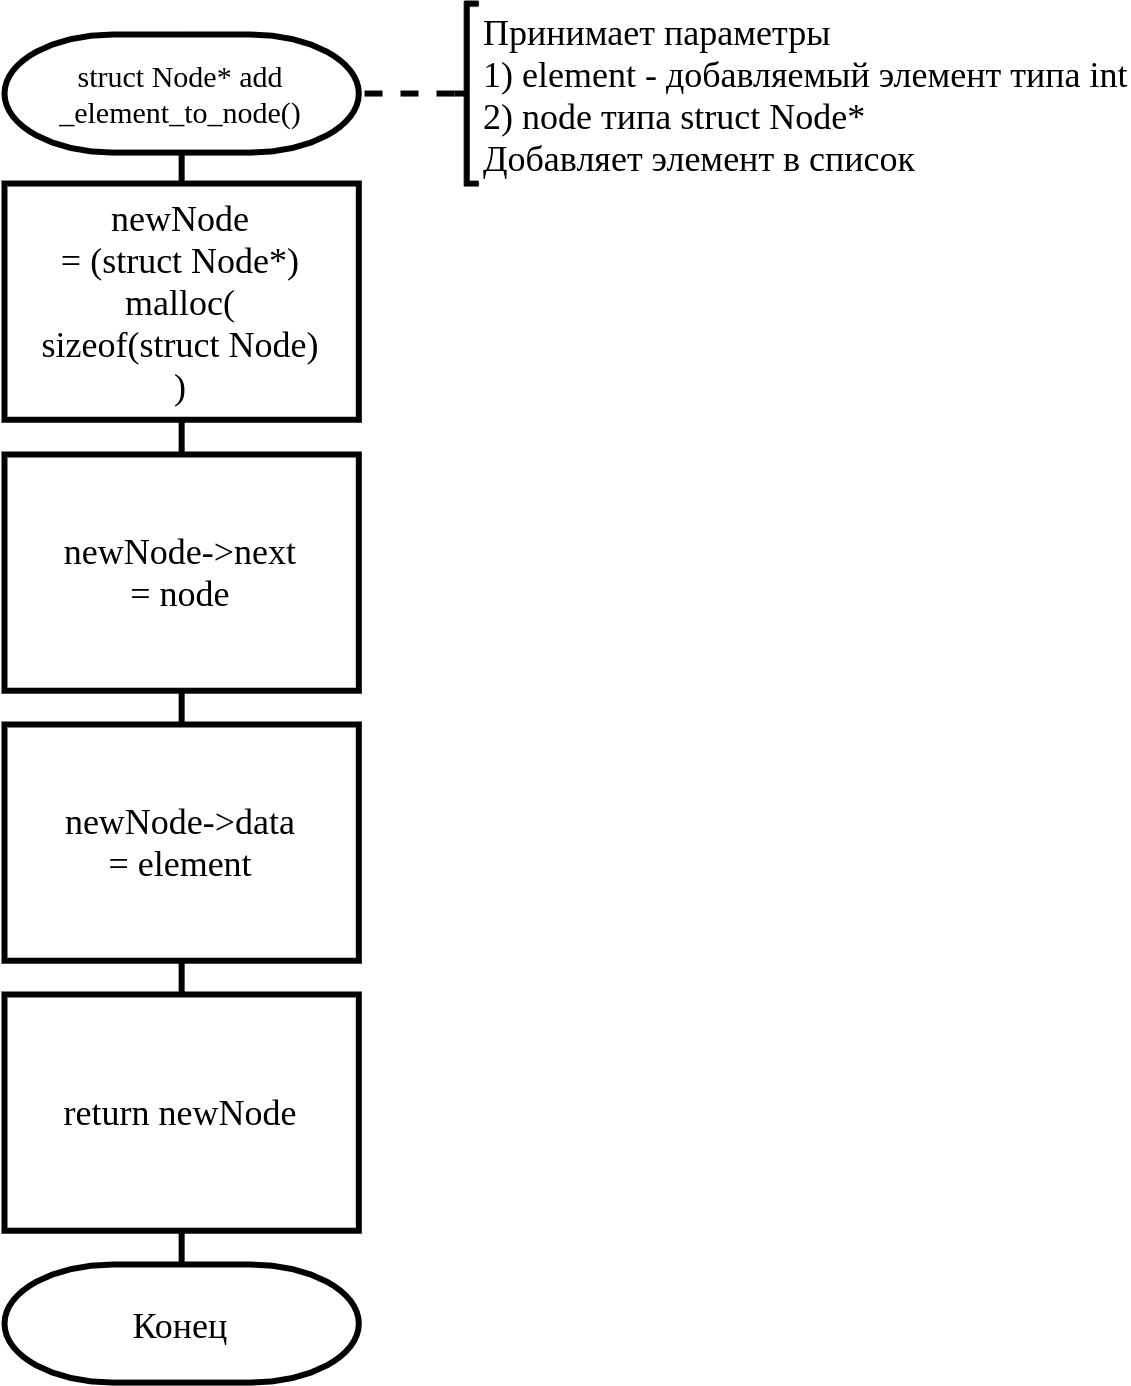
\includegraphics[]{../src/add_element_to_node/add_element_to_node.png}
    }
    \caption{add\_element\_to\_node()}
    \label{fig:add_element_to_node}
\end{figure}

\lstinputlisting[
    language=C,
    name=add\_element\_to\_node.c
]{../src/add_element_to_node/add_element_to_node.c}

\lstinputlisting[
    language=C,
    name=add\_element\_to\_node.h
]{../src/add_element_to_node/add_element_to_node.h}

% = = = = = = = = = = =

\subsection{get\_list\_size()}

Блок-схема на рисунке \ref{fig:get_list_size}.

\begin{figure}[pht]
    \center{
        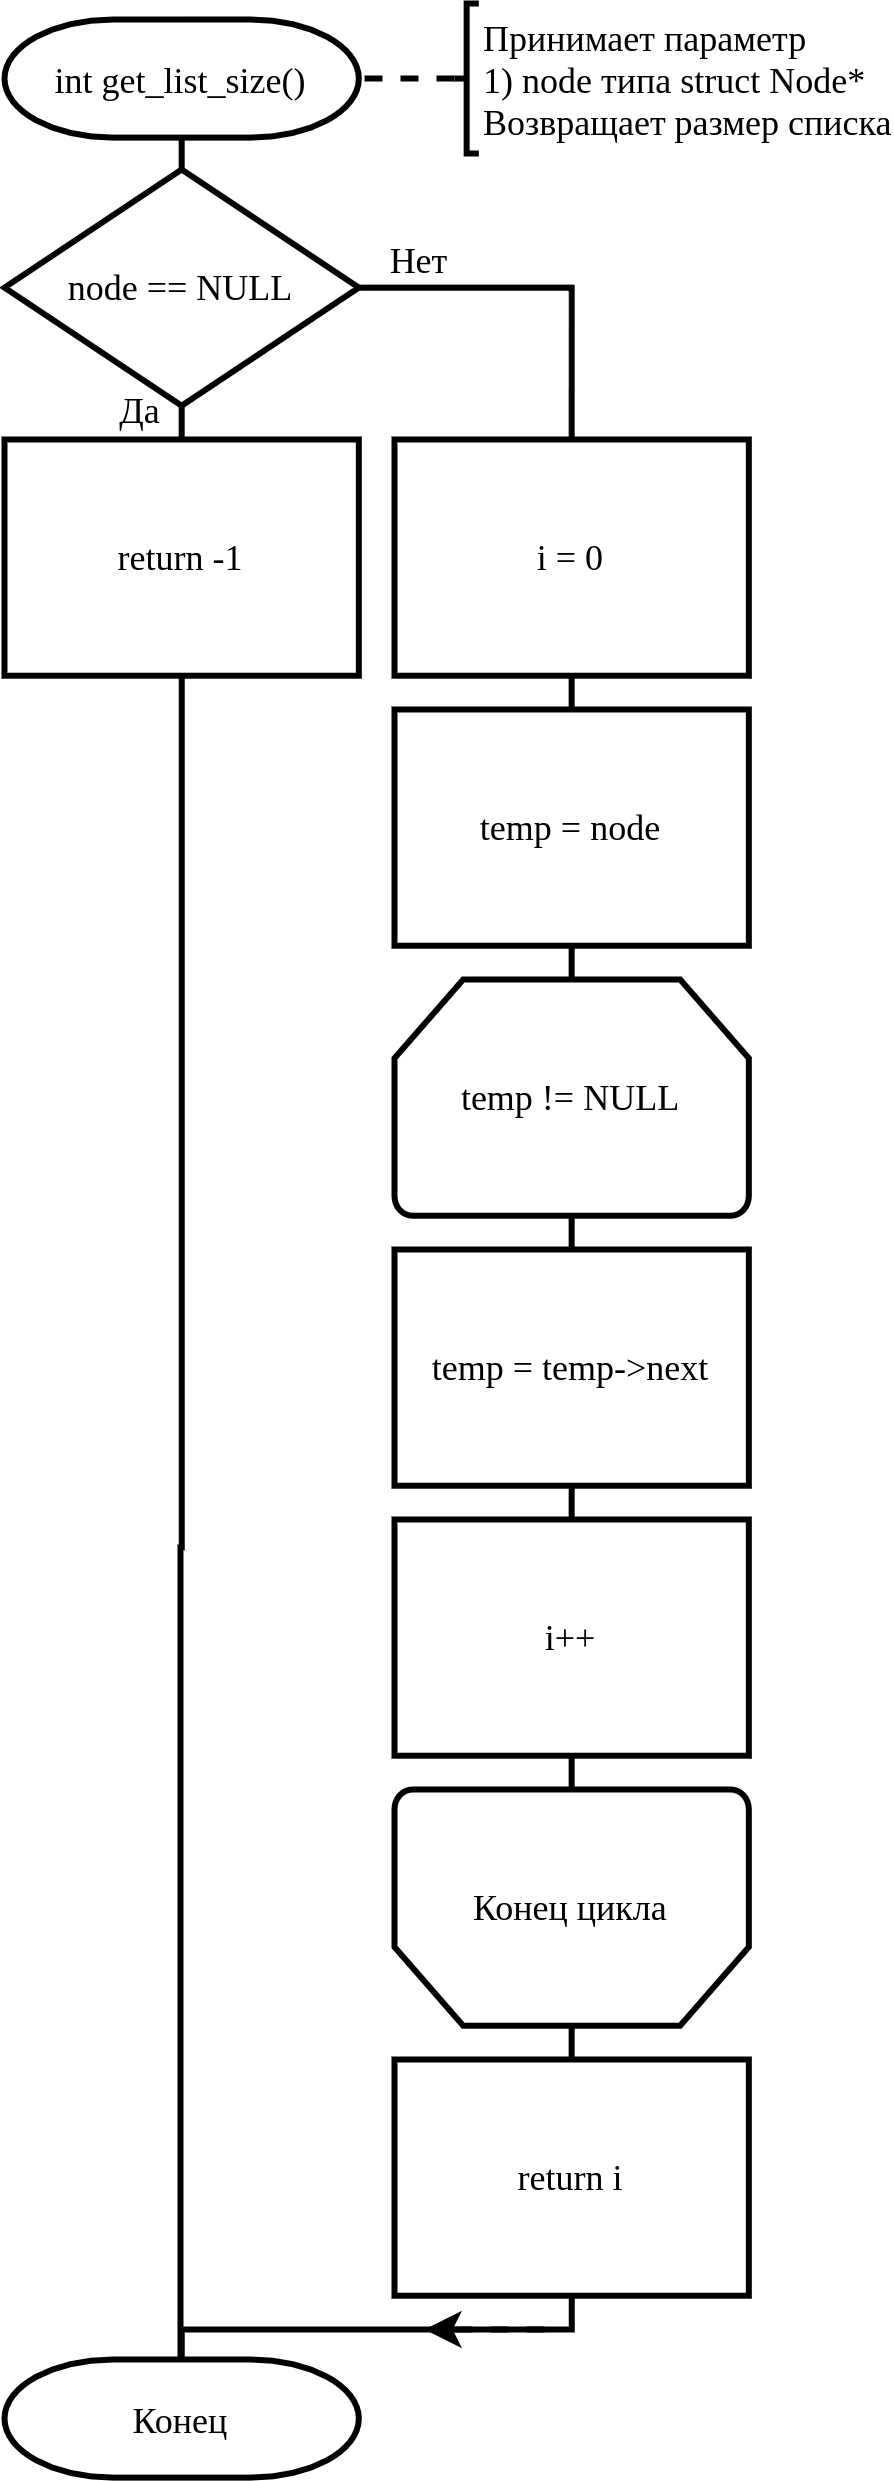
\includegraphics[]{../src/get_list_size/get_list_size.png}
    }
    \caption{get\_list\_size()}
    \label{fig:get_list_size}
\end{figure}

\lstinputlisting[
    language=C,
    name=get\_list\_size.c
]{../src/get_list_size/get_list_size.c}

\lstinputlisting[
    language=C,
    name=get\_list\_size.h
]{../src/get_list_size/get_list_size.h}

% = = = = = = = = = = =

\subsection{print\_list()}

Блок-схема на рисунке \ref{fig:print_list}.

\begin{figure}[pht]
    \center{
        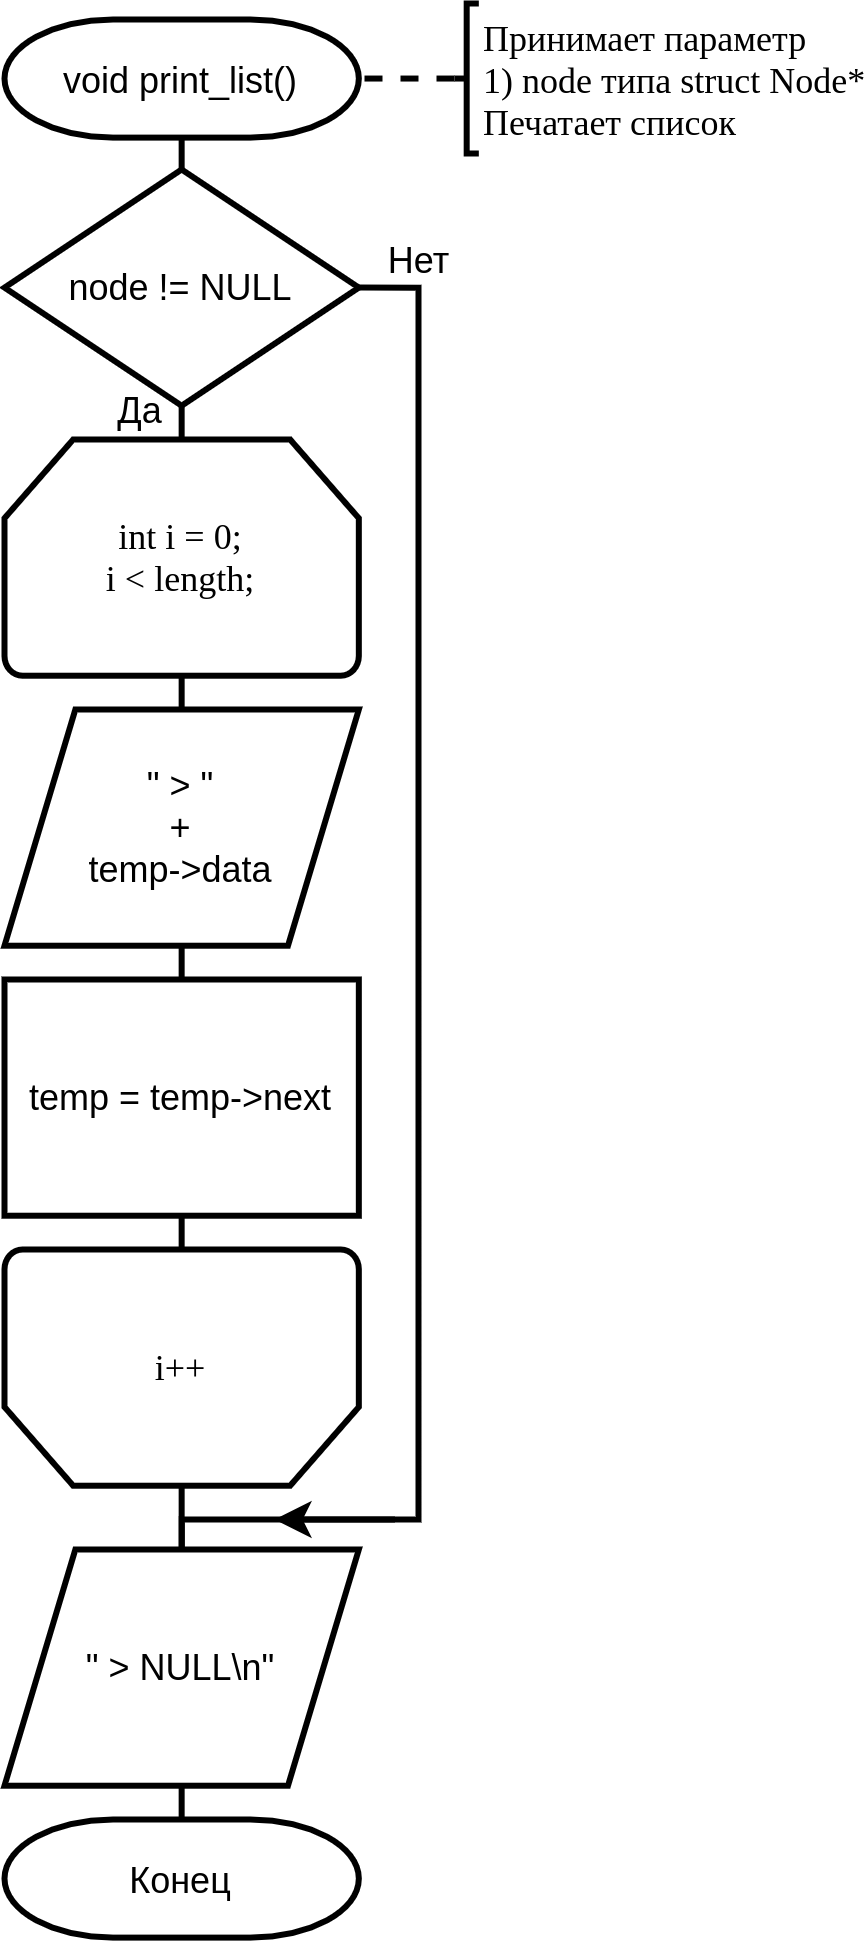
\includegraphics[]{../src/print_list/print_list.png}
    }
    \caption{print\_list()}
    \label{fig:print_list}
\end{figure}

\lstinputlisting[
    language=C,
    name=print\_list.c
]{../src/print_list/print_list.c}

\lstinputlisting[
    language=C,
    name=print\_list.h
]{../src/print_list/print_list.h}

% = = = = = = = = = = =

\subsection{clear\_list()}

Блок-схема на рисунке \ref{fig:clear_list}.

\begin{figure}[pht]
    \center{
        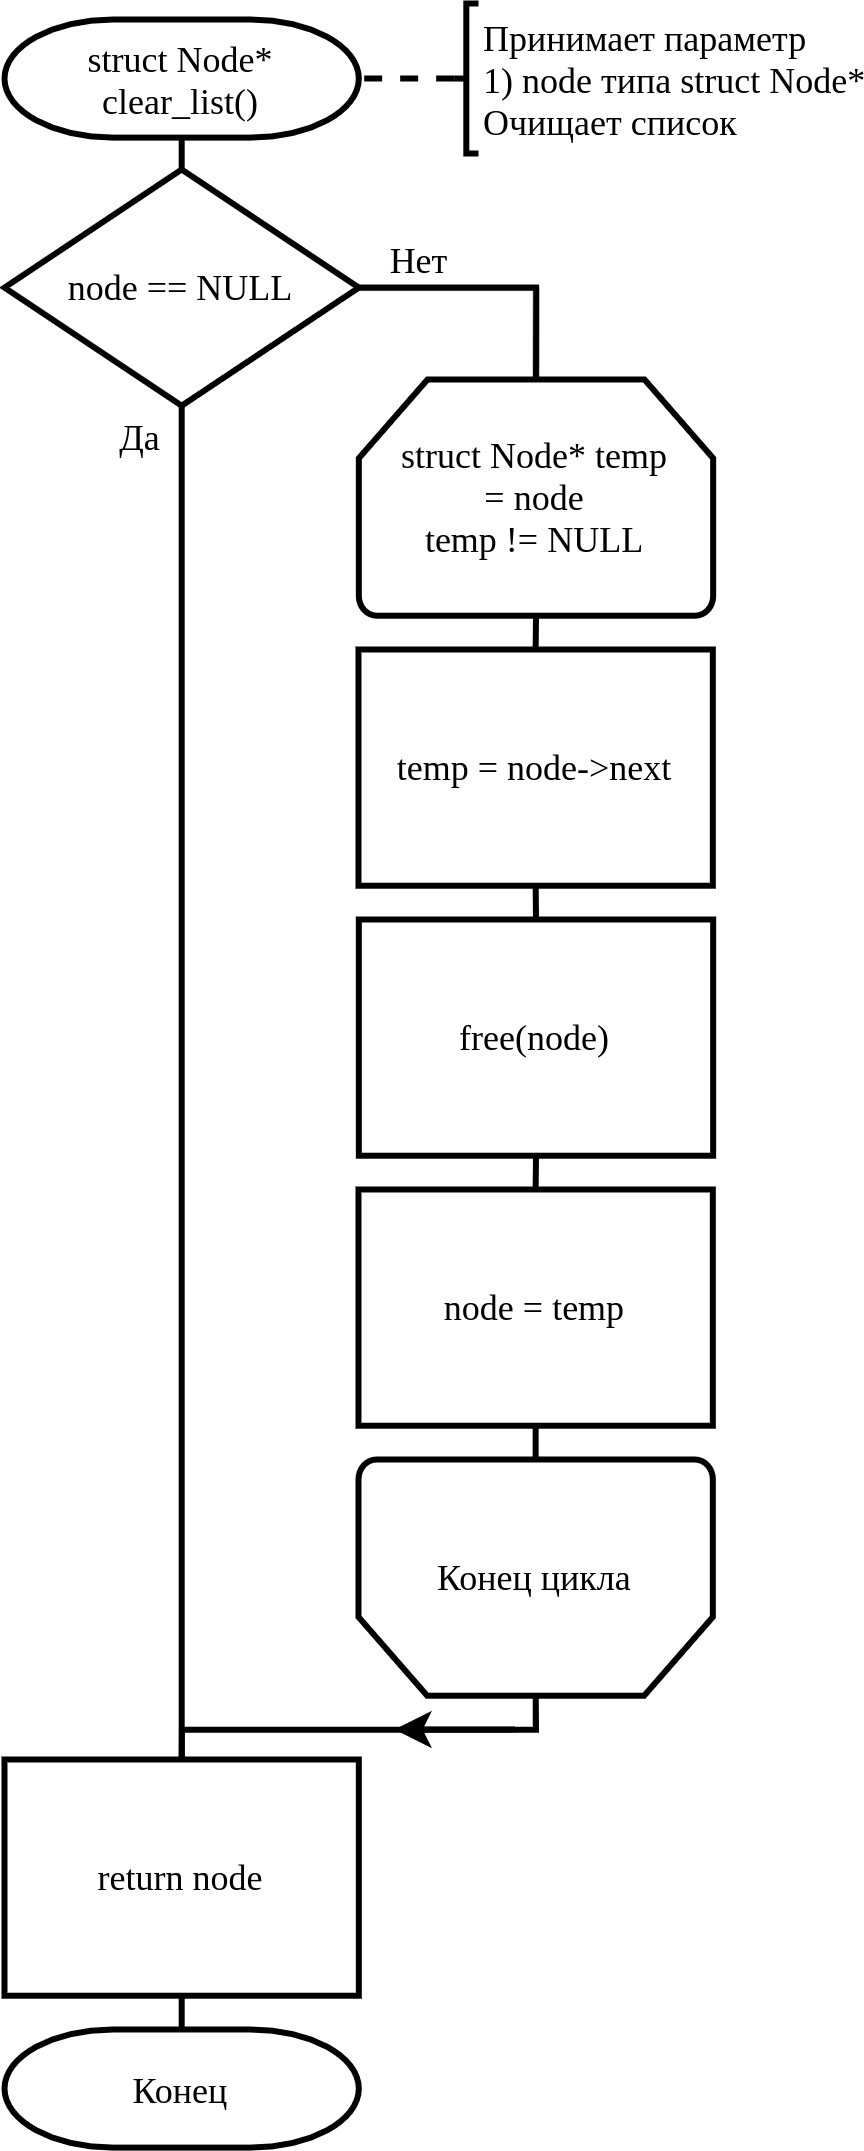
\includegraphics[]{../src/clear_list/clear_list.png}
    }
    \caption{clear\_list()}
    \label{fig:clear_list}
\end{figure}

\lstinputlisting[
    language=C,
    name=clear\_list.c
]{../src/clear_list/clear_list.c}

\lstinputlisting[
    language=C,
    name=clear\_list.h
]{../src/clear_list/clear_list.h}
%===>>>

\section{Тестирование}

\textbf{Тест 1:} <<Если списка 1 нет в списке 2>>

\underline{Ожидаемый результат:} список 2 не измениться

\underline{Описание:} При цикличном обходе не найдёт сходства списка 1 и списка 2, то есть список 2 не поменяется

\underline{Полученный результат:} не изменённый список

\underline{Вывод:} получение списка работает корректно

\begin{tcolorbox}
\begin{verbatim}
Test 1
Дано:
queue 1: > 400 > 300 > 200 > 100 > NULL
queue 2: > 444444 > 333333 > 400 > 300 > 200 > 222222 > 111111 > NULL
queue 3: > 99001122 > 55667788 > 11223344 > NULL
Получить: изменённый список 2 (Если список 1 есть в списке 2,
то заменить его списком 3)
queue 3: > NULL
Ответ: (список 2) > 444444 > 333333 > 400 > 300 > 200 > 222222
> 111111 > NULL
queue 1: > NULL
queue 2: > NULL
\end{verbatim}
\end{tcolorbox}

\textbf{Тест 2:} <<Если список 1 есть в списке 2>>

\underline{Ожидаемый результат:} список 2 измениться

\underline{Описание:} При цикличном обходе найдётся сходства списка 1 и списка 2, то есть список 2 поменяется

\underline{Полученный результат:} изменённый список

\underline{Вывод:} получение нового списка работает корректно

\begin{tcolorbox}
\begin{verbatim}
Test 2
Дано:
queue 1: > 4 > 3 > 2 > 1 > NULL
queue 2: > 300 > 200 > 4 > 3 > 2 > 4 > 3 > 2 > 4 > 3 > 2 > 4 > 3 > 2 > 1 >
111 > 100 > NULL
queue 3: > 444444444 > 33333333 > 22222222 > NULL
Получить: изменённый список 2 (Если список 1 есть в списке 2,
то заменить его списком 3)
Ответ: (список 2) > 300 > 200 > 4 > 3 > 2 > 4 > 3 > 2 > 4 > 3 > 2 >
444444444 > 33333333 > 22222222 > 111 > 100 > NULL
queue 1: > NULL
queue 2: > NULL
\end{verbatim}
\end{tcolorbox}

\textbf{Тест 3:} <<Если список 1 встречается несколько раз в списке 2>>

\underline{Ожидаемый результат:} список 2 измениться

\underline{Описание:} При цикличном обходе у нас списко 3 соединяется указателями, что не вогодно. Нужно реализовывать через добавление элементов

\underline{Полученный результат:} изменённый список

\underline{Вывод:} работает не корректно. Цикл в бесконечности. Нужно исправлять

\begin{tcolorbox}
\begin{verbatim}
Test 3
Дано:
queue 1: > 1 > 2 > NULL
queue 2: > 0 > 0 > 0 > 1 > 2 > 0 > 0 > 1 > 2 > 0 > 0 > NULL
queue 3: > 33333 > 44444 > 55555 > NULL
Получить: изменённый список 2 (Если список 1 есть в списке 2,
то заменить его списком 3)
\end{verbatim}
\end{tcolorbox}

%<<<===Вывод ЛР
\labconclusion{Научились работать с динамической памятью. Изучили динамическую структуру данных: списки.}
%===>>>

\end{document}